\chapter{СТРУКТУРНО-ПАРАМЕТРИЧЕСКИЙ СИНТЕЗ ПОЗИЦИОННЫХ ЭЛЕКТРОПНЕВМАТИЧЕСКИХ ПРИВОДОВ С ДИСКРЕТНЫМ УПРАВЛЕНИЕМ}\label{ch:ch5}

\section{Постановка задачи структурно-параметрического синтеза пневмопривода}

Структурно-параметрический синтез позиционного пневмопривода с дискретными распределителями
представляет собой комплексную задачу, предполагающую выбор оптимальной структуры управления и определение её
параметров для обеспечения требуемых показателей качества работы системы. Особенностью данной задачи является
необходимость учёта противоречивых требований к статико-динамическим и ресурсным показателям пневмопривода,
что предопределяет её многокритериальный характер.

Требования к позиционному пневмоприводу с дискретными распределителями могут
быть формализованы в виде совокупности критериев, отражающих различные аспекты его функционирования.
Исходя из проведённого в предыдущих главах анализа, основные требования к системе могут быть разделены на три ключевые группы:

\begin{enumerate}
	\item \textbf{Требования к точности позиционирования}, выражаемые через предельно допустимую ошибку в
	      установившемся режиме $\Delta x_{\text{доп}}$.
	\item \textbf{Требования к качеству переходного процесса}, включающие ограничения по быстродействию
	      $t_{\text{п}} \leq t_{\text{п.доп}}$, перерегулированию $\sigma \leq \sigma_{\text{доп}}$ и другим динамическим показателям.
	\item \textbf{Ресурсные требования}, характеризующие интенсивность
	      переключений распределителей $N_{\text{перекл}} \leq N_{\text{перекл.доп}}$ за цикл позиционирования.
\end{enumerate}

Таким образом, обобщённая постановка задачи структурно-параметрического
синтеза может быть представлена следующим образом:
\begin{equation}
	F_{\text{опт}} = \text{arg}\,\text{min}_{S \in \mathbf{S}, \mathbf{p} \in \mathbf{P}_S} \mathbf{J}(S, \mathbf{p}),
\end{equation}
где $F_{\text{опт}}$ -- оптимальная конфигурация пневмопривода;
$S$ -- структура системы управления из множества допустимых структур $\mathbf{S}$;
$\mathbf{p}$ -- вектор параметров выбранной структуры управления из множества допустимых значений $\mathbf{P}_S$;
$\mathbf{J}(S, \mathbf{p})$ -- векторный критерий оптимальности.
\nomenclature{$F_{\text{опт}}$}{Оптимальная конфигурация пневмопривода\nomrefeqpage}
\nomenclature{$S$}{Структура системы управления\nomrefeqpage}
\nomenclature{$\mathbf{p}$}{Вектор параметров выбранной структуры управления\nomrefeqpage}
\nomenclature{$\mathbf{J}(S, \mathbf{p})$}{Векторный критерий оптимальности\nomrefeqpage}

Для различных структур управления необходимо определить соответствующие векторы варьируемых параметров:
\begin{itemize}
	\item для ПИД-регулятора с ШИМ: $\mathbf{p}_{\text{ПИД}} = [K_p, K_i, K_d, f_{\text{ШИМ}}, K_{\text{т}}]^T$;
	\item для управления в скользящих режимах с интегральной поверхностью: $\mathbf{p}_{\text{УСР-И}} = [\lambda_1, \lambda_2, \varepsilon_1, \varepsilon_2, \ldots, \varepsilon_n]^T$;
	\item для управления в скользящих режимах с терминальной поверхностью: $\mathbf{p}_{\text{УСР-Т}} = [\beta, \gamma, p, q, \varepsilon_1, \varepsilon_2, \ldots, \varepsilon_n]^T$;
	\item для нечёткого управления: $\mathbf{p}_{\text{НУ}} = [\mathbf{x}_m, \mathbf{y}_m, \mathbf{z}_m, \mathbf{w}]^T$;
	\item для прогнозного управления: $\mathbf{p}_{\text{MPC}} = [N_p, N_u, Q, R, \Delta t]^T$.
\end{itemize}
где компоненты векторов представляют собой настраиваемые параметры соответствующих алгоритмов управления, описанные в главе 3.

Для оценки эффективности функционирования различных структур
пневмопривода с дискретными распределителями необходимо определить
количественные критерии, отражающие основные требования к системе.
В рамках данного исследования в качестве критериев оптимизации предлагается использовать точность позиционирования,
интегральный критерий качества переходного процесса и интенсивность переключений распределителей.

\textbf{Точность позиционирования ($AC$).}
Критерий точности позиционирования характеризует статическую ошибку системы в установившемся режиме и определяется как:
\begin{equation}
	AC = \lim_{t \to \infty} |e(t)| = \lim_{t \to \infty} |x_{\text{зад}} - x(t)|,
\end{equation}
где $x_{\text{зад}}$ -- заданное положение, а $x(t)$ -- текущее положение штока пневмоцилиндра.

На практике, учитывая конечное время моделирования $T_{\text{мод}}$, данный критерий вычисляется как:
\begin{equation}
	AC = |e(T_{\text{мод}})| = |x_{\text{зад}} - x(T_{\text{мод}})|,
\end{equation}
при условии, что время моделирования выбрано достаточно большим для достижения установившегося состояния.
\nomenclature{$AC$}{Точность позиционирования}

\textbf{Интегральный критерий качества переходного процесса ($ITAE$).}
Для оценки качества переходного процесса предлагается использовать интегральный критерий с учётом времени и модуля ошибки:
\begin{equation}
	ITAE = \int_0^{T_{\text{мод}}} t |e(t)| dt,
\end{equation}
где $t$ -- время, $|e(t)|$ -- модуль ошибки позиционирования.
\nomenclature{$ITAE$}{Интегральный критерий качества переходного процесса}

Данный критерий обеспечивает комплексную оценку динамических свойств системы, учитывая как
быстродействие, так и характер затухания переходного процесса. Использование модуля ошибки
позволяет адекватно оценивать качество процессов с колебаниями относительно установившегося значения.

\textbf{Интенсивность переключений распределителей ($SI$).}
Для оценки ресурсных показателей системы предлагается критерий,
характеризующий интенсивность переключений распределителей:
\begin{equation}
	SI = \sum_{i=1}^4 N_i,
\end{equation}
где $N_i$ -- количество переключений $i$-го распределителя за цикл позиционирования.
\nomenclature{$SI$}{Интенсивность переключений распределителей}

Данный критерий напрямую связан с ресурсом электромагнитных клапанов и общей надёжностью системы.
Минимизация интенсивности переключений способствует увеличению срока службы пневмопривода и снижению эксплуатационных затрат.

Ключевой особенностью рассматриваемой задачи является наличие противоречий между представленными критериями
оптимизации. Данные противоречия обусловлены физическими особенностями пневмопривода с дискретными распределителями и проявляются в следующих взаимосвязях:

\begin{enumerate}
	\item \textbf{Противоречие между точностью позиционирования и интенсивностью переключений.} Повышение
	      точности позиционирования ($AC \to \min$) требует более частого переключения распределителей
	      для точной коррекции положения штока, что приводит к увеличению $SI$.

	\item \textbf{Противоречие между качеством переходного процесса и интенсивностью переключений.}
	      Улучшение динамических характеристик системы ($ITAE \to \min$) обычно достигается за счёт
	      более агрессивного управления, что также увеличивает число переключений $SI$.

	\item \textbf{Взаимосвязь между точностью и качеством переходного процесса.} Данная взаимосвязь более сложная и может иметь
	      различный характер в зависимости от структуры управления. В некоторых случаях улучшение динамических
	      характеристик способствует повышению точности, в других -- между этими критериями также возникает противоречие.
\end{enumerate}

Помимо указанных взаимосвязей, при решении задачи структурно-параметрического
синтеза необходимо учитывать ряд ограничений:

\begin{enumerate}
	\item \textbf{Конструктивные ограничения} на параметры пневмопривода,
	      связанные с физическими свойствами системы:
	      \begin{equation}
		      \mathbf{g}_{\text{конст}}(\mathbf{p}) \leq 0,
	      \end{equation}
	      где $\mathbf{g}_{\text{конст}}$ -- вектор-функция конструктивных ограничений.

	\item \textbf{Ограничения на параметры алгоритмов управления}, определяемые
	      требованиями к устойчивости системы и реализуемости алгоритмов:
	      \begin{equation}
		      \mathbf{p}_{\min} \leq \mathbf{p} \leq \mathbf{p}_{\max},
	      \end{equation}
	      где $\mathbf{p}_{\min}$ и $\mathbf{p}_{\max}$ -- векторы минимальных и максимальных значений параметров.

	\item \textbf{Ограничения на показатели качества системы}, задаваемые техническим заданием:
	      \begin{equation}
		      \begin{aligned}
			      AC   & \leq AC_{\text{доп}}   \\
			      ITAE & \leq ITAE_{\text{доп}} \\
			      SI   & \leq SI_{\text{доп}}
		      \end{aligned}
	      \end{equation}
\end{enumerate}

Учитывая многокритериальный характер задачи и наличие противоречий между критериями,
целесообразно применить подход, основанный на выявлении множества Парето-оптимальных решений,
которые представляют собой компромисс между различными критериями. При этом выбор конкретного
решения из множества Парето-оптимальных будет зависеть от приоритетов конкретной задачи позиционирования.

Таким образом, задача структурно-параметрического синтеза пневмопривода может быть сформулирована как
нахождение множества Парето-оптимальных решений для различных структур управления и
последующий выбор наилучшей структуры и её параметров на основе заданных приоритетов задачи.

\section{Построение фронтов Парето для различных управляющих структур}

Наличие нескольких критериев оптимизации требует решения вопроса выбора
предпочтительной структуры на основании сравнения фронтов Парето, построенных
для каждой конкурсной структуры. Использование традиционных методов построения
множества Парето приводит к необходимости проведения многократных расчетов с
использованием сложных динамических моделей. Это существенно увеличивает трудоемкость
процесса получения решения и делает процесс затратным по времени.

Для решения этой проблемы было предложено использование замещающих суррогатных
моделей (surrogate models) \cite{surrogate_model} при построении фронтов Парето.
Данные модели строятся на основании исходных моделей и способны с достаточной
точностью аппроксимировать зависимость критериев оптимизации от параметров
пневмопривода. Основная цель использования суррогатных
моделей заключается в снижении вычислительных затрат при поиске Парето-оптимальных
решений за счёт замены трудоёмкого полного моделирования более быстрой аппроксимацией

Проведенный анализ (приложение \ref{app:choosing-the-best-surrogate-model-method}) показал,
что наиболее предпочтительно в качестве суррогатной модели использовать нейронную сеть с
глубокой архитектурой, включающей остаточные связи (residual connections)
для улучшения сходимости при обучении. Основным строительным
блоком такой сети является резидуальный блок, описываемый следующими уравнениями \cite{he2015deepresiduallearningimage}:

\begin{equation}
	\mathbf{h}_1 = \phi(\mathbf{W}_1 \mathbf{x} + \mathbf{b}_1),
\end{equation}
\begin{equation}
	\mathbf{h}_2 = \mathbf{W}_2 \mathbf{D}(\mathbf{h}_1) + \mathbf{b}_2,
\end{equation}
\begin{equation}
	\mathbf{y} = \phi(\mathbf{h}_2 + \mathbf{W}_s \mathbf{x}),
\end{equation}
где $\mathbf{x}$ -- входной вектор параметров управляющей структуры;
$\mathbf{W}_1, \mathbf{W}_2, \mathbf{W}_s$ -- весовые матрицы;
$\mathbf{b}_1, \mathbf{b}_2$ -- векторы смещения;
$\phi(\cdot)$ -- функция активации (ReLU);
$\mathbf{D}(\cdot)$ -- функция прореживания (Dropout) с вероятностью \num{0.1};
$\mathbf{y}$ -- выходной вектор резидуального блока.
\nomenclature{$\mathbf{x}$}{Вектор параметров управляющей структуры\nomrefeqpage}
\nomenclature{$\mathbf{y}$}{вектор резидуального блока\nomrefeqpage}
\nomenclature{$\mathbf{h}_1$}{Выходной вектор первого резидуального блока\nomrefeqpage}
\nomenclature{$\mathbf{h}_2$}{Выходной вектор второго резидуального блока\nomrefeqpage}
\nomenclature{$\mathbf{W}_1, \mathbf{W}_2, \mathbf{W}_s$}{Весовые матрицы\nomrefeqpage}
\nomenclature{$\mathbf{b}_1, \mathbf{b}_2$}{Векторы смещения\nomrefeqpage}
\nomenclature{$\phi(\cdot)$}{Функция активации\nomrefeqpage}
\nomenclature{$\mathbf{D}(\cdot)$}{Функция прореживания\nomrefeqpage}


Полная архитектура суррогатной модели включает последовательность резидуальных блоков
с увеличением размерности скрытых слоёв и заключительный линейный слой
для предсказания значений критериев оптимизации:

\begin{equation}
	\mathbf{y} = f(\mathbf{x}) = \mathbf{W}_\text{out} \cdot \text{RB}_n(\text{RB}_{n-1}(...\text{RB}_1(\mathbf{x})...)) + \mathbf{b}_\text{out},
\end{equation}
где $\text{RB}_i$ -- $i$-й резидуальный блок;
$\mathbf{W}_\text{out}, \mathbf{b}_\text{out}$ -- параметры выходного слоя;
$n$ -- количество резидуальных блоков, определяемое в процессе оптимизации гиперпараметров.

Использование нейросетевых суррогатных моделей при построении фронтов Парето
требует решения вопросов предварительного обучения нейросети на основании серии
расчетов по исходной модели (рисунок \ref{fig:process-diagram}). Для этого в пространстве
параметров формируется выборка данных (расчетные точки) на основании
которых в результате численного моделирования по исходной модели
рассчитываются показатели качества.

\begin{figure}[h]
	\centering
	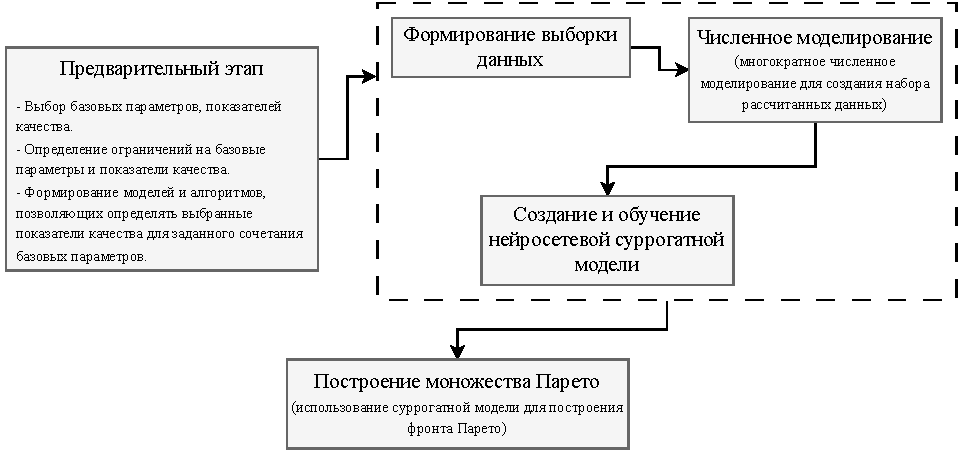
\includegraphics[width=\textwidth]{part5/диаграмма-процесса-формирования.pdf}
	\caption{Алгоритм построения фронта Парето}
	\label{fig:process-diagram}
	
\end{figure}

Для сокращения вычислительных затрат количество расчетных точек должно быть минимальным,
но достаточным для обеспечения необходимой точности замещающей модели.
Кроме того, точки должны быть равномерно распределены в пространстве параметров.

Были исследованы различные методы заполнения пространства параметров: равномерная сетка,
случайная выборка, метод латинского гиперкуба (Latin Hypercube Sampling, LHS) и метод Соболя.
Для количественной оценки равномерности покрытия пространства параметров был разработан метрический метод \cite{pub21},
основанный на сравнении удельного среднего расстояния между соседними точками.
Коэффициент Монте-Карло рассчитывался по формуле:

\begin{equation}
	I = \frac{0,5}{\sqrt{\frac{n}{A}}},
\end{equation}
где $n$ -- количество реальных точек, $A$ -- площадь области, в рассматриваемом случае $A = 1$.

Результаты расчета данного коэффициента для различных методов выборки представлены в таблице~\ref{tab:monte_carlo_coefficient}.

\begin{table}[ht]
	\centering
	\caption{Сравнение равномерности покрытия пространства параметров различными методами выборки}
	\label{tab:monte_carlo_coefficient}
    \small
	\begin{tabular}{lc}
		\midrule
		\textbf{Метод выборки}     & \textbf{Коэффициент Монте-Карло} \\
		\midrule
		Равномерная сетка          & 0,947                            \\
		Случайная выборка          & 1,024                            \\
		Метод латинского гиперкуба & 0,997                            \\
		Метод Соболя               & 0,980                            \\
		\midrule
	\end{tabular}
\end{table}

Как следует из таблицы, метод латинского гиперкуба (LHS) характеризуется
оптимальным значением коэффициента Монте-Карло,
что свидетельствует о наименьшей дисперсии расстояний между соседними точками и, соответственно,
о более равномерном заполнении пространства параметров. На рисунке \ref{fig:fill_field} представлены
примеры заполнения пространства параметров различными методами выборки.

\begin{figure}[ht]
	\centering
	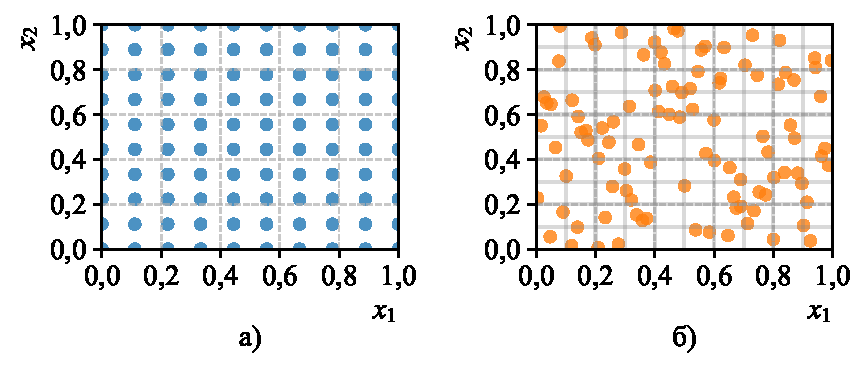
\includegraphics{part5/lhs_vs_grid.pdf}
	\caption{Заполнение пространства параметров различными методами выборки:\\
		a) равномерная сетка; б) метод латинского гиперкуба}
	\label{fig:fill_field}
\end{figure}

На основе проведенного анализа для формирования обучающей выборки данных при построении
суррогатных моделей был выбран метод латинского гиперкуба. 
Применение LHS позволило сформировать эффективную выборку из 2500 комбинаций базовых параметров, что
привело к снижению трудоемкости построения множества Парето и сокращению времени расчета на 48\%.
Использование выборки, сформированной методом латинского гиперкуба, обеспечило среднюю точность
замещающей суррогатной модели на уровне 91\% при максимальном отклонении 12\%.

Каждый эксперимент характеризуется вектором параметров $\mathbf{p}_i$ и соответствующим вектором
значений критериев оптимизации $\mathbf{J}_i = [AC_i, ITAE_i, SI_i]^T$. Общая обучающая выборка
представляет собой набор пар $\{(\mathbf{p}_i, \mathbf{J}_i)\}_{i=1}^N$, где $N$ -- общее число экспериментов.

Для повышения качества суррогатной модели проводится нормализация
входных и выходных данных с использованием стандартного масштабирования:

\begin{equation}
	\mathbf{p}_\text{норм} = \frac{\mathbf{p} - \boldsymbol{\mu}_p}{\boldsymbol{\sigma}_p},
\end{equation}
\begin{equation}
	\mathbf{J}_\text{норм} = \frac{\mathbf{J} - \boldsymbol{\mu}_J}{\boldsymbol{\sigma}_J},
\end{equation}
где $\boldsymbol{\mu}_p, \boldsymbol{\sigma}_p$ -- векторы средних значений и стандартных отклонений для параметров;
$\boldsymbol{\mu}_J, \boldsymbol{\sigma}_J$ -- векторы средних значений и стандартных отклонений для критериев.

Для повышения надёжности и точности предсказаний использовался ансамбль из нескольких суррогатных
моделей с различными начальными условиями. Каждая модель обучается минимизации взвешенной среднеквадратичной ошибки:

\begin{equation}
	\mathcal{L}(\mathbf{W}, \mathbf{b}) = \frac{1}{N} \sum_{i=1}^N w_i \cdot \|\mathbf{J}_{\text{норм},i} - f(\mathbf{p}_{\text{норм},i}; \mathbf{W}, \mathbf{b})\|_2^2,
\end{equation}
где $w_i$ -- весовой коэффициент для $i$-го образца;
$\mathbf{W}, \mathbf{b}$ -- обобщённые весовые матрицы и векторы смещения сети.

Для оптимизации параметров нейронной сети используется алгоритм AdamW с
начальной скоростью обучения $\eta = 10^{-3}$ и регуляризацией весов $\lambda = 10^{-4}$.
Для адаптивной настройки скорости обучения применяется циклический планировщик
(Cyclic Learning Rate Scheduler) с треугольным режимом изменения скорости.

Тренировка выполняется в течение заданного числа эпох (обычно 1000) с
мониторингом ошибки на валидационном наборе для предотвращения переобучения. Валидационный
набор формируется методом кросс-валидации (K-Fold Cross Validation) с K = 5.

Прогноз ансамбля моделей формируется как
среднее значение предсказаний отдельных моделей:

\begin{equation}
	\hat{\mathbf{J}}(\mathbf{p}) = \frac{1}{M} \sum_{m=1}^M f_m(\mathbf{p}),
\end{equation}
где $M$ -- количество моделей в ансамбле;
$f_m(\mathbf{p})$ -- предсказание $m$-й модели.

Для определения оптимальной архитектуры суррогатной модели проводится поиск гиперпараметров
с использованием байесовской оптимизации. В качестве оптимизируемых гиперпараметров рассматриваются:

\begin{itemize}
	\item Скорость обучения $\eta \in [10^{-4}, 10^{-2}]$
	\item Размерность первого скрытого слоя $h_1 \in [2, 64]$
	\item Размерность второго скрытого слоя $h_2 \in [2, 64]$
\end{itemize}

Целевой функцией оптимизации является средняя ошибка валидации при К-кратной перекрёстной
проверке. Байесовская оптимизация использует гауссовский процесс для построения вероятностной
модели зависимости ошибки валидации от гиперпараметров и последовательно выбирает точки в
пространстве гиперпараметров для максимизации ожидаемого улучшения (Expected Improvement).

После обучения ансамбля суррогатных моделей осуществляется поиск
Парето-оптимальных решений с использованием эволюционного алгоритма
многокритериальной оптимизации NSGA-III (Non-dominated Sorting Genetic Algorithm III).
Данный алгоритм для эффективного решения многокритериальных задач с большим числом
целевых функций.

Алгоритм NSGA-III основан на следующих принципах:
\begin{enumerate}
	\item Недоминируемая сортировка популяции решений на фронты.
	\item Использование опорных точек (reference points) для сохранения разнообразия решений вдоль фронта Парето.
	\item Эволюционные операторы селекции, скрещивания и мутации для исследования пространства решений.
\end{enumerate}

В результате проведения многокритериальной оптимизации были получены фронты Парето для 
позиционных пневмоприводов различной структуры, отражающие взаимосвязь между тремя
ключевыми критериями: точностью позиционирования ($AC$), интегральным критерием качества
($ITAE$) и интенсивностью переключений распределителей ($SI$).

\textbf{Парето-фронт для пневмопривода с модифицированным ПИД-регулятором и ШИМ.}
При исследовании ПИД-регулятора с ШИМ варьировались пять параметров: $K_p$, $K_i$, $K_d$,
частота ШИМ $f_{\text{ШИМ}}$ и коэффициент адаптивного торможения $K_{\text{т}}$.

Парето-фронт для ПИД-регулятора с ШИМ имеет относительно гладкую структуру без характерных
разрывов, что свидетельствует о плавном изменении свойств системы при варьировании параметров.
Минимальная точность позиционирования составляет 0,41 мм при значении динамического критерия $ITAE = 0,0305$ \si{\metre\per\second\square}
и интенсивности переключений $SI = 35$ переключений. При снижении требований к точности до 1,5 \si{\milli\metre} снижается
интенсивность переключений до $SI = 26$ при незначительном ухудшении динамики ($ITAE = 0,04$ \si{\metre\per\second\square}).

Характерной особенностью является небольшой диапазон изменения $ITAE$ (от 0,0298 до 0,0427 \si{\metre\per\second\square}) при значительном изменении
точности (от 0,41 до 2,57 мм), что указывает на ограниченные возможности ПИД-регулятора с ШИМ в
обеспечении высокой точности при сохранении приемлемых динамических характеристик.
На рисунке \ref{fig:pid_pareto} представлена поврерхность Пратео-фротна.
\begin{figure}[h]
	\centering
	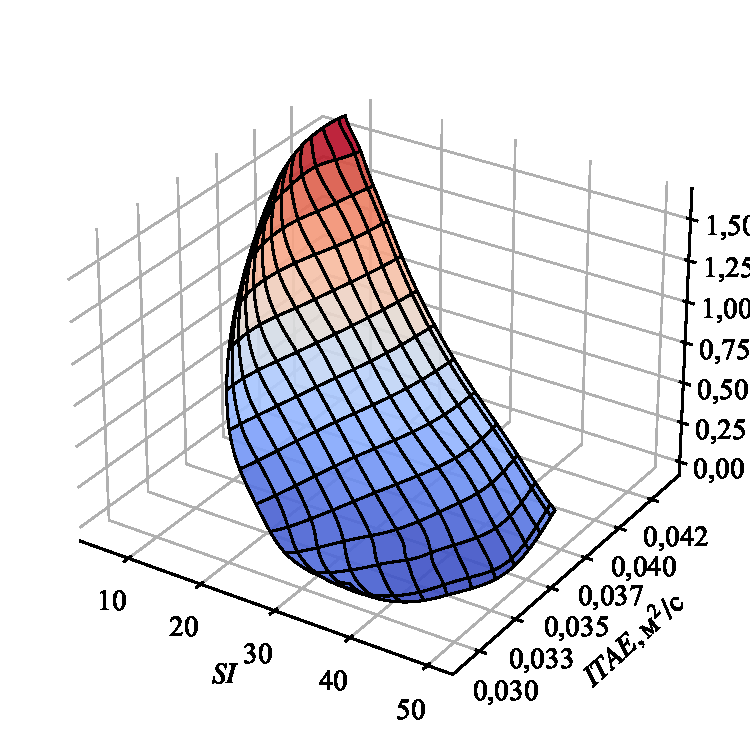
\includegraphics{part5/fronts/ПИД+ШИМ.pdf}
	\caption{Парето-фронт для ПИШ с ШИМ}
	\label{fig:pid_pareto}
\end{figure}

\textbf{Парето-фронты для пневмопривода с управлением в скользящих режимах.}
Исследование проводилось для комбинаций типов поверхностей скольжения (интегральная и терминальная)
и количества режимов управления (три, пять и семь).

Для трехрежимного управления с интегральной поверхностью (УСР-И-3) минимальная
точность составляет 0,8 мм при $ITAE = 0,051$ \si{\metre\per\second\square} и $SI = 20$
Характерной особенностью является разрыв в области $SI = 20$, указывающий на существование различных локально-оптимальных конфигураций.

Пятирежимное управление (УСР-И-5) обеспечивает значительное
улучшение: точность 0,36 мм при $ITAE = 0,033$ \si{\metre\per\second\square} и $SI = 5$.

Семирежимное управление с интегральной поверхностью (УСР-И-7) показывает
наилучшую точность 0,13 мм при $ITAE = 0,019$ \si{\metre\per\second\square} и $SI = 15$.

Трехрежимное управление с терминальной поверхностью (УСР-Т-3)
обеспечивает точность 0,31 мм, что в 2,5 раз лучше по сравнению с
интегральной поверхностью при том же количестве режимов. Пятирежимное
управление с терминальной поверхностью (УСР-Т-5) дает точность 0,28 мм при $ITAE = 0,019$
\si{\metre\per\second\square} и $SI = 10$.

Семирежимное управление с терминальной поверхностью (УСР-Т-7) обеспечивает
точность 0,13 мм при $ITAE = 0,024$ \si{\metre\per\second\square} и $SI = 15$.

Сравнительный анализ показывает, что терминальная поверхность обеспечивает более высокую точность
при малом числе режимов, но при увеличении числа режимов преимущество
становится менее выраженным. Для обоих типов поверхностей наиболее значительный скачок качества происходит при переходе от трех к пяти режимам.

На рисунке \ref{fig:scrolling_pareto} представлен Парето-фронт для УСР-И-3
\begin{figure}[h]
	\centering
	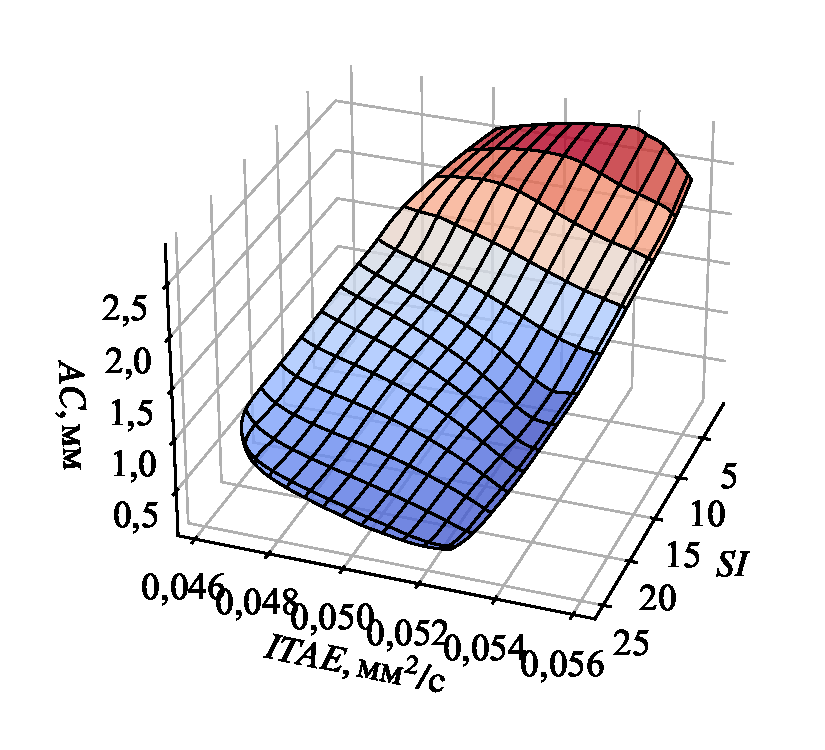
\includegraphics{part5/fronts/УСР-И-3.pdf}
	\caption{Парето-фронт для УСР-И-3}
	\label{fig:scrolling_pareto}
\end{figure}

\textbf{Парето-фронт для пневмопривода с нечетким управлением.}
При исследовании нечеткого управления варьировались формы
функций принадлежности, их расположение и конфигурация базы правил.

Парето-фронт для нечеткого регулятора имеет гладкую структуру.
Минимальная точность составляет 0,40 мм при $ITAE = 0,0551$ \si{\metre\per\second\square} и $SI = 23$,
что демонстрирует высокую эффективность нечеткого управления в обеспечении отличных динамических характеристик.

На рисунке \ref{fig:fuzzy_pareto} представлен Парето-фронт для нечеткого регулятора.
\begin{figure}[h]
	\centering
	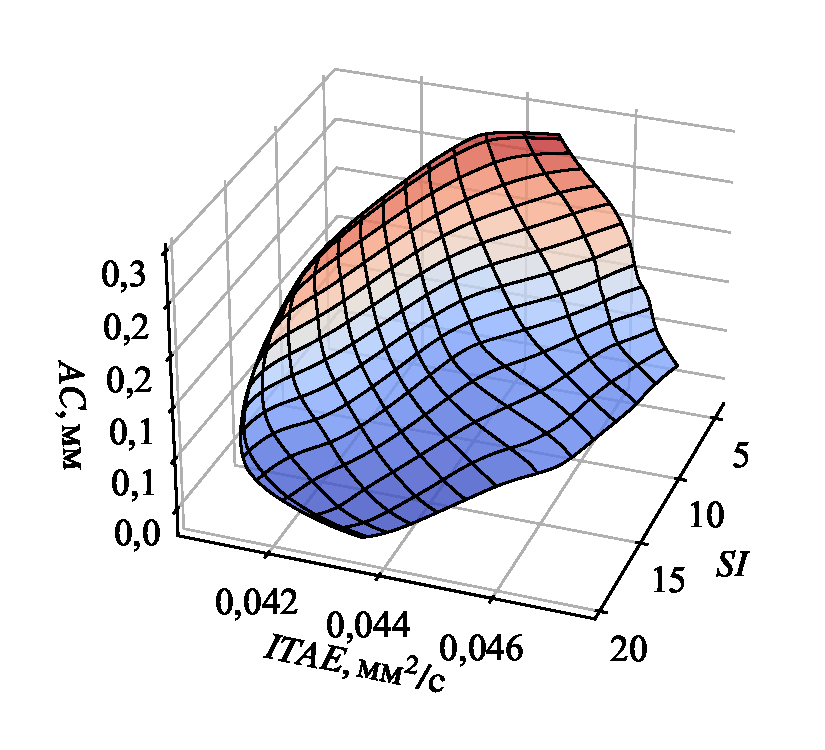
\includegraphics{part5/fronts/Нечеткий.pdf}
	\caption{Парето-фронт для нечеткого регулятора}
	\label{fig:fuzzy_pareto}
\end{figure}

\textbf{Парето-фронт для пневмопривода с прогнозным управлением.}
При исследовании прогнозного управления (MPC) варьировались горизонт прогноза,
горизонт управления, весовые коэффициенты целевой функции, параметры внутренней модели и шаг дискретизации.

Парето-фронт для MPC имеет ярко выраженную ступенчатую структуру с отчетливыми
кластерами решений. В области высокой точности (0,12 мм) наблюдается кластер
при $ITAE = 0,032$ \si{\metre\per\second\square} и $SI = 14$~--~$16$.

На рисунке \ref{fig:mpc_pareto} представлен Парето-фронт для MPC.
\begin{figure}[h]
	\centering
	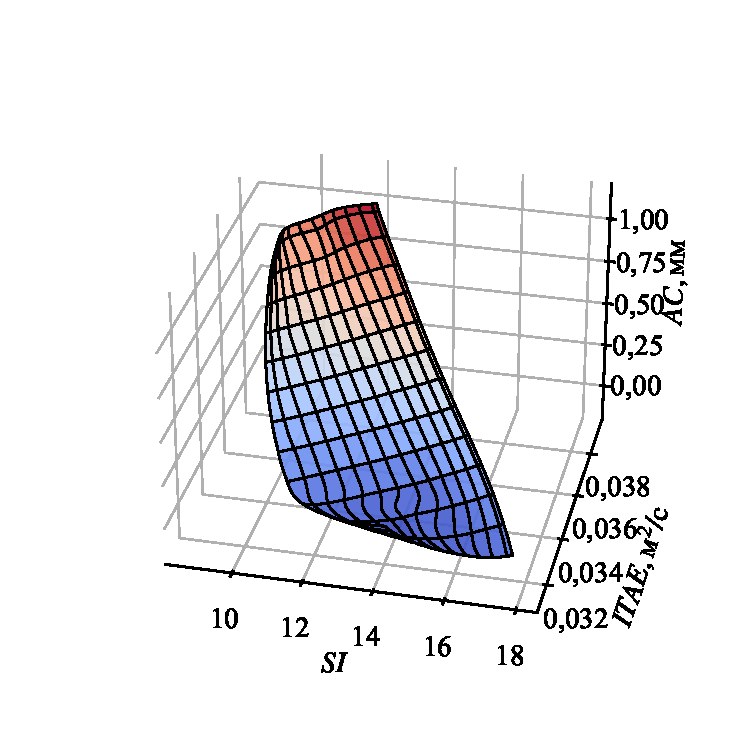
\includegraphics{part5/fronts/MPC.pdf}
	\caption{Парето-фронт для MPC}
	\label{fig:mpc_pareto}
\end{figure}

После формирования фронтов Парето для каждой конкурсной структуры
была проведена оценка точности построения границы Парето по суррогатной
модели. Для этого на сформированном фронте Парето равномерно выбирался
набор точек. Для каждой точки определялись значения вектора параметров,
соответствующего каждой точке. Далее производился расчет показателей качества
по исходной модели и сравнение результатов расчета со значениями,
соответствующими точкам на фронте Парето. 

Для количественной оценки погрешностей использовались следующие показатели:
\begin{enumerate}
	\item Относительная погрешность для каждого критерия:
	      \begin{equation}\label{eq:relative_error}
		      \delta_{\text{rel},i} = \frac{|y_i^{\text{факт}} - y_i^*|}{|y_i^*|} \cdot 100\%
	      \end{equation}

	\item Средняя относительная погрешность по всем критериям:
	      \begin{equation}\label{eq:mean_relative_error}
		      \delta_{\text{rel}} = \frac{1}{m} \sum_{i=1}^{m} \frac{|y_i^{\text{факт}} - y_i^*|}{|y_i^*|} \cdot 100\%
	      \end{equation}
	      где $m$ -- число критериев (в данном случае $m = 3$).

	\item Нормализованная абсолютная погрешность:
	      \begin{equation}\label{eq:normalized_absolute_error}
		      \delta_{\text{abs},i} = \frac{|y_i^{\text{факт}} - y_i^*|}{y_{i,\max} - y_{i,\min}} \cdot 100\%
	      \end{equation}

	\item Средняя нормализованная абсолютная погрешность:
	      \begin{equation}\label{eq:mean_normalized_absolute_error}
		      \delta_{\text{abs}} = \frac{1}{m} \sum_{i=1}^{m} \frac{|y_i^{\text{факт}} - y_i^*|}{y_{i,\max} - y_{i,\min}} \cdot 100\%
	      \end{equation}
\end{enumerate}

На рисунке~\ref{fig:verification_diagram} представлена лепестковая диаграмма
средних относительных погрешностей для конкурсных структур пневмопривода.
Из диаграммы видно, что наименьшая погрешность характерна для ПИД-регулятора с
ШИМ и нечеткого управления, что объясняется более плавной функциональной зависимостью
между параметрами и критериями в этих структурах. Наибольшая погрешность наблюдается
для семирежимного управления в скользящих режимах с терминальной поверхностью, что
связано с высокой нелинейностью и сложностью параметрической оптимизации этой структуры.

\begin{figure}[h]
	\centering
	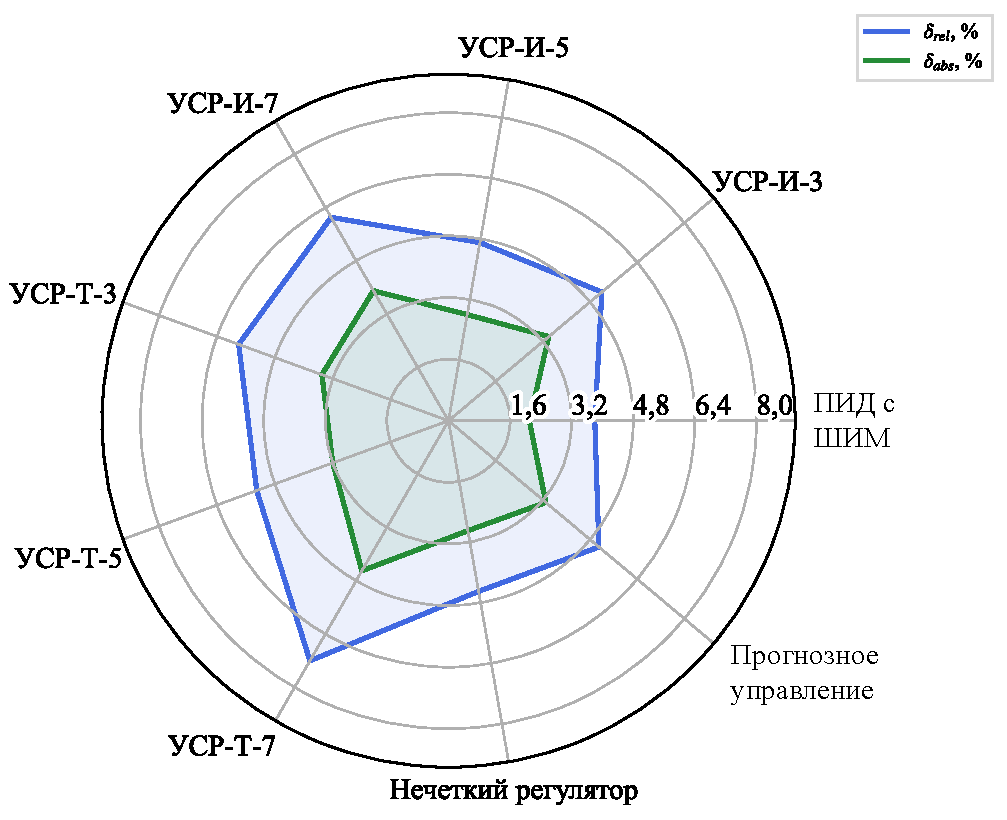
\includegraphics{part5/diagramm_error.pdf}
	\caption{Сравнение средних относительных погрешностей для различных конкурсных структур}
	\label{fig:verification_diagram}
\end{figure}

В таблице~\ref{tab:verification_results} приведены численные результаты
проверки применимости методики для различных управляющих структур.

\begin{table}[ht]
	\centering
	\caption{Результаты проверки применимости методики решения обратной задачи}
	\label{tab:verification_results}
	\small
	\begin{tabular}{lccc}
		\midrule
		\textbf{Метод управления} & $\delta_{\text{rel}}$,~\% & $\delta_{\text{abs}}$,~\% & \textbf{Максимальная погрешность}~\% \\
		\midrule
		ПИД-регулятор с ШИМ       & \num{3.8}                 & \num{2.1}                 & \num{9.2}                            \\
		УСР-И-3                   & \num{5.2}                 & \num{3.4}                 & \num{11.6}                           \\
		УСР-И-5                   & \num{4.7}                 & \num{2.8}                 & \num{10.3}                           \\
		УСР-И-7                   & \num{6.1}                 & \num{3.9}                 & \num{13.5}                           \\
		УСР-Т-3                   & \num{5.8}                 & \num{3.5}                 & \num{12.7}                           \\
		УСР-Т-5                   & \num{5.3}                 & \num{3.2}                 & \num{11.9}                           \\
		УСР-Т-7                   & \num{7.2}                 & \num{4.5}                 & \num{15.8}                           \\
		Нечеткий регулятор        & \num{4.5}                 & \num{2.9}                 & \num{10.8}                           \\
		Прогнозное управление     & \num{5.1}                 & \num{3.3}                 & \num{12.5}                           \\
		\midrule
	\end{tabular}
\end{table}

Для проверки применимости методики для различных требований к критериям проведен
дополнительный анализ, в ходе которого тестовые точки были разделены на группы по преобладающим требованиям:
\begin{itemize}
	\item Группа А -- приоритет точности позиционирования (малые значения $AC$).
	\item Группа Б -- приоритет динамических характеристик (малые значения $ITAE$).
	\item Группа В -- приоритет ресурсосбережения (малые значения $SI$).
	\item Группа Г -- сбалансированные требования ко всем критериям.
\end{itemize}

Результаты анализа показали, что методика наиболее эффективна для группы Г (сбалансированные требования),
где средняя относительная погрешность составила \num{4.2}\%. Для групп А, Б и В средние
относительные погрешности составили \num{5.7}\%, \num{4.9}\% и \num{5.5}\% соответственно.
Это свидетельствует о том, что методика обеспечивает приемлемую точность во всем диапазоне
требований, однако более эффективна при сбалансированных требованиях к критериям.
\section{Выбор структуры и оптимальных параметров пневмопривода}\label{sec:inverse_optimization}

Построенные фронты Парето устанавливают предельно достижимые значения
критериев качества для каждой структуры. Для примера на рисунке \ref{fig:pareto_fronts_two}
изображены фронты Парето, соответствующие двум структурам пневмопривода (УСР-И-7 и УСР-Т-7)
и построенные для двух показателей качества $SI$ и $ITAE$ при $AC = \num{0.6}\text{мм}$. Оптимальное решение
всегда лежит на поверхности, огибающей фронты Парето. Выбор
структуры связан с поиском проектировщиком наиболее приемлемого сочетания
показателей качества на этой огибающей и определения структуры, чей фронт
Парето включает точку, соответствующую этому сочетанию.

\begin{figure}[h]
	\centering
	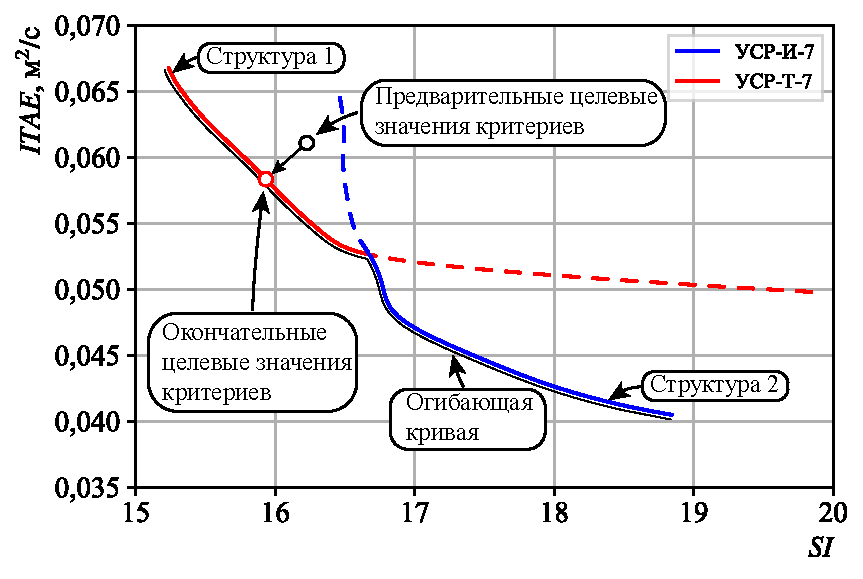
\includegraphics{part5/contour_comparison.pdf}
	\caption{Фронты Парето для двух структур пневмопривода}
	\label{fig:pareto_fronts_two}
\end{figure}
	

Данный подход позволяет проектировщику наглядно видеть цену
увеличения того или иного показателя качества за счет снижения
остальных, что позволяет более обоснованно назначать их целевые
значения. Кроме того, возможно улучшение предварительно заданных
целевых значений критериев качества до их предельно достижимых уровней.

Выбор окончательных целевых значений критериев качества может
быть осуществлено нахождением ближайшей точки на огибающей фронтов
Парето от точки, соответствующей предварительно назначенным целевым значениям (рисунок \ref{fig:pareto_fronts_two}).

Поскольку критерии имеют различную физическую природу и масштабы, для корректного определения
расстояния необходимо выполнить их нормализацию.
В данной работе используется нормализация относительно диапазона изменения каждого критерия:

\begin{equation}\label{eq:normalization}
	\tilde{y}_i = \frac{y_i - y_{i,\min}}{y_{i,\max} - y_{i,\min}}, \quad i \in \{AC, ITAE, SI\},
\end{equation}
где $y_{i,\min}$ и $y_{i,\max}$ -- минимальное и максимальное значения $i$-го критерия на фронте Парето.

В качестве меры расстояния между нормализованными векторами критериев используется взвешенная евклидова норма:

\begin{equation}\label{eq:weighted_norm}
	\|\mathbf{\tilde{y}}(\mathbf{p}) - \mathbf{\tilde{y}}^*\|_w = \sqrt{\sum_{i} w_i (\tilde{y}_i(\mathbf{p}) - \tilde{y}_i^*)^2},
\end{equation}
где $w_i$ -- весовые коэффициенты, отражающие относительную важность критериев.

Для практической реализации описанной выше методики разработан алгоритм поиска ближайшей точки
на фронте Парето к заданной целевой точке. Алгоритм включает предварительную обработку данных,
эффективный поиск ближайшей точки и дополнительную интерполяцию для повышения точности.

Перед началом поиска выполняется предварительная обработка данных, включающая следующие шаги:
\begin{enumerate}
	\item Фильтрация точек фронта Парето для исключения доминируемых точек, которые
	      могли появиться из-за численных погрешностей в процессе построения фронта.

	\item Вычисление диапазонов изменения критериев $[y_{i,\min}, y_{i,\max}]$ для каждого критерия $i$.
	\item Нормализация критериев для всех точек фронта Парето и целевой точки согласно уравнению~\eqref{eq:normalization}.
	\item Формирование пространственной структуры данных для эффективного поиска ближайших точек.
\end{enumerate}

Поиск ближайшей к целевой точки на фронте Парето осуществляется в два этапа:

\begin{enumerate}
	\item Грубый поиск -- вычисление расстояний от целевой точки до всех точек фронта Парето
	      и выбор точки с минимальным расстоянием. Этот этап необходим для определения начального приближения.
	\item Уточняющий поиск -- локальная оптимизация в окрестности найденной точки с использованием
	      кубической интерполяции. Данный этап позволяет более точно определить параметры управления в
	      случае, если оптимальное решение находится между точками фронта Парето.
\end{enumerate}

Для грубого поиска используется прямое вычисление расстояний по формуле~\eqref{eq:weighted_norm} и выбор точки с минимальным значением:

\begin{equation}\label{eq:brute_force_search}
	j^* = \arg\min_{j \in \{1,\ldots,N\}} \|\mathbf{\tilde{y}}^{(j)} - \mathbf{\tilde{y}}^*\|_w,
\end{equation}
где $\mathbf{\tilde{y}}^{(j)}$ -- вектор нормализованных критериев для $j$-й точки фронта Парето;
$N$ -- общее число точек на фронте.

Для уточняющего поиска используется квадратичная интерполяция параметров управления в
окрестности найденной точки. Пусть $\mathbf{p}^{(j^*)}$ -- вектор параметров управления;
соответствующий найденной ближайшей точке фронта Парето.
Тогда интерполированные параметры вычисляются следующим образом:

\begin{equation}\label{eq:interpolation}
	\mathbf{p}^* = \mathbf{p}^{(j^*)} + \sum_{k \in K} \alpha_k (\mathbf{p}^{(k)} - \mathbf{p}^{(j^*)}),
\end{equation}
где $K$ -- множество индексов ближайших соседей точки $j^*$;
$\alpha_k$ -- весовые коэффициенты, определяемые на основе расстояний до целевой точки:

\begin{equation}\label{eq:interpolation_weights}
	\alpha_k = \frac{(d_{j^*} - d_{\min})^2}{\sum_{l \in K} (d_l - d_{\min})^2} \cdot \frac{d_{\min}}{d_k},
\end{equation}
где $d_k = \|\mathbf{\tilde{y}}^{(k)} - \mathbf{\tilde{y}}^*\|_w$ -- расстояние от $k$-й точки до целевой точки;
$d_{\min} = \min_{k \in K} d_k$ -- минимальное расстояние среди рассматриваемых точек.

Найденное положение точки с окончательными целевыми значениями
критериев качества на огибающей кривой может быть уточнено экспертно.
Данное положение однозначно определяет наиболее предпочтительную структуру
по принадлежности этой точки фронту Парето той или иной структуры. 

Далее для выбранной структуры и вектора целевых значений критериев качества
требуется найти соответствующий вектор параметров оптимизации. 
Поскольку при построении фронта Парето было получено соответствие
рассчитанных точек фронта Парето и параметров оптимизации, то решение
этой задачи сводится к построению интерполяционной зависимости и
нахождению по ней значений параметров по известным значениям критериев качества.

После определения оптимальных значений параметров целесообразно провести перерасчет
критериев качества по исходной модели. Если полученные в результате моделирования значения
критериев существенно отличаются от целевых, что может быть вызвано нелинейностью зависимостей
между параметрами и критериями, выполняется коррекция параметров.

Коррекция основана на методе последовательных приближений:

\begin{equation}\label{eq:parameters_correction}
	\mathbf{p}^{(n+1)} = \mathbf{p}^{(n)} + \beta (\mathbf{y}^* - \mathbf{y}^{(n)}) \cdot \frac{\partial \mathbf{y}}{\partial \mathbf{p}}|_{\mathbf{p}^{(n)}},
\end{equation}
где $\mathbf{p}^{(n)}$ -- вектор параметров на $n$-й итерации;
$\mathbf{y}^{(n)}$ -- соответствующий вектор критериев;
$\beta$ -- коэффициент коррекции.
$\frac{\partial \mathbf{y}}{\partial \mathbf{p}}|_{\mathbf{p}^{(n)}}$ -- матрица частных производных критериев по параметрам, оцениваемая численно.
\nomenclature{$\mathbf{y}^{(n)}$}{Вектор критериев на $n$-й итерации\nomrefeqpage}
\nomenclature{$\frac{\partial \mathbf{y}}{\partial \mathbf{p}}|_{\mathbf{p}^{(n)}}$}{Матрица частных производных критериев по параметрам\nomrefeqpage}
\nomenclature{$\beta$}{Коррекционный коэффициент\nomrefeqpage}
\nomenclature{$\mathbf{p}^{(n+1)}$}{Вектор параметров на $(n+1)$-й итерации\nomrefeqpage}

Итерационный процесс коррекции продолжается до тех пор, пока не будет достигнута
требуемая точность соответствия критериев целевым значениям или не будет выполнено максимальное число итераций.
\section{Практические рекомендации по выбору управляющих структур пневмопривода с дискретными распределителями}

На основе проведенного анализа фронтов Парето были разработаны практические рекомендации
по выбору оптимальных управляющих структур позиционного пневмопривода с дискретными
распределителями в зависимости от типовых предъявляемых требований,
характерных для  конкретных технических задач.

Для наглядного представления предпочтительных областей применения различных
структур управления разработана карта, отображающая эффективность алгоритмов
управления в зависимости от двух ключевых параметров: требуемой точности
позиционирования и ресурсосбережения согласно рисунку~\ref{fig:algorithm_map}.

\begin{figure}[ht]
	\centering
	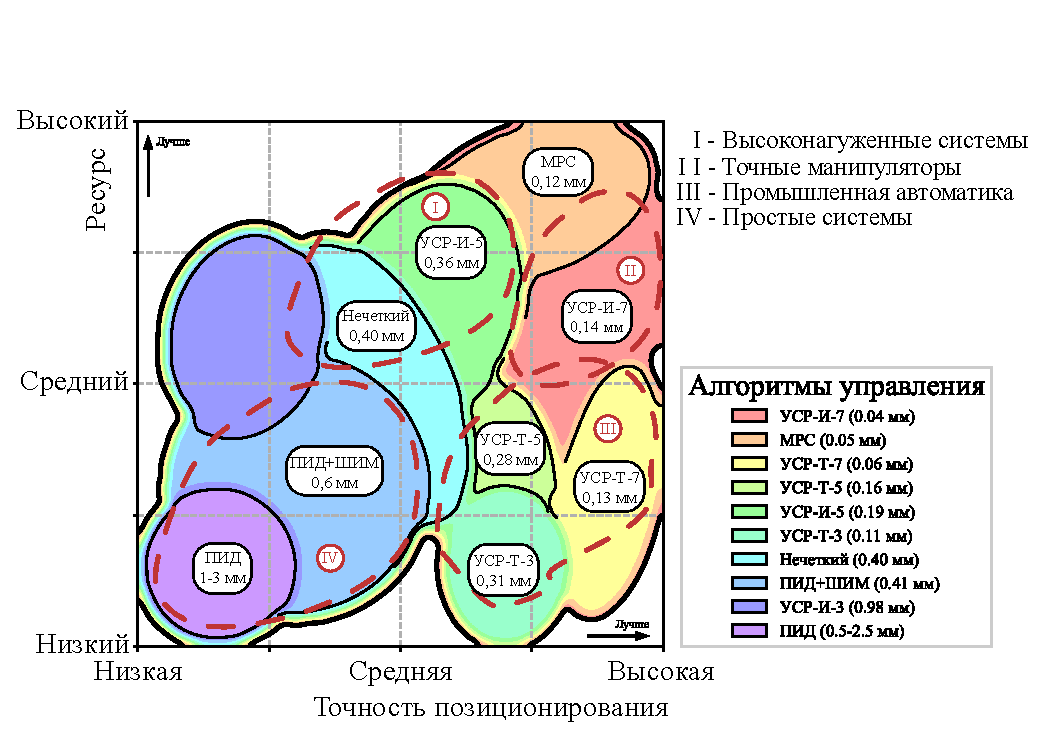
\includegraphics{part5/Карта.eps}
	\caption{Карта предпочтительных областей применения алгоритмов управления:
		горизонтальная ось отражает требуемые динамические качества, вертикальная
		-- ресурсосбережение (минимизацию числа переключений распределителей)}
	\label{fig:algorithm_map}
\end{figure}

На карте предпочтительных областей выделены следующие зоны применения:

\begin{enumerate}
	\item \textbf{Область высоконагруженных систем} (средняя точность позиционирования и
	      высокое ресурсосбережение) -- преимущественная область применения пятирежимного управления
	      в скользящих режимах с интегральной поверхностью (УСР-И-5, 0,36 мм) и прогнозного
	      управления (MPC, 0,12 мм). Эти алгоритмы обеспечивают баланс между точностью
	      позиционирования и высоким ресурсосбережением.

	\item \textbf{Область точных манипуляторов} (высокая точность и высокий ресурс) -- эффективное
	      применение семирежимного управления в скользящих режимах с интегральной поверхностью
	      (УСР-И-7, 0,14 мм), обеспечивающего наивысшую точность позиционирования при сохранении
	      высокого ресурсосбережения.

	\item \textbf{Область промышленной автоматики} (высокая точность и средний ресурс) -- оптимальное
	      использование терминального управления в скользящих режимах (УСР-Т-5, 0,28 мм; УСР-Т-7, 0,13 мм),
	      обеспечивающего хорошую точность позиционирования при средних показателях ресурсосбережения.

	\item \textbf{Область простых систем} (низкая точность и низкие требования к ресурсу) -- рациональное
	      применение ПИД-регулятора (0,5-2,5 мм), ПИД-регулятора с ШИМ (0,6 мм) и трехрежимного управления
	      в скользящих режимах (УСР-И-3, 0,8-1 мм), обеспечивающих невысокую точность позиционирования при
	      низких требованиях к ресурсосбережению.
\end{enumerate}

При выборе алгоритма управления также следует учитывать динамические характеристики
систем через интегральный критерий $ITAE$. Наилучшие показатели по данному критерию
обеспечивают нечеткое управление (0,006 м$\cdot$с²), прогнозное управление (0,012 м$\cdot$с²)
и семирежимное управление в скользящих режимах с интегральной поверхностью (0,019 м$\cdot$с²).

На основе проведенных исследований выработаны конкретные рекомендации по выбору
параметров различных алгоритмов управления для типовых задач позиционирования.
Рекомендуемые значения параметров систематизированы в таблице~\ref{tab:recommended_parameters}.

\begin{table}[ht]
	\centering
	\caption{Рекомендуемые параметры управляющих структур для типовых задач позиционирования}
	\label{tab:recommended_parameters}
	\scriptsize
	\begin{tabular}{p{3.5cm}p{3cm}p{4cm}p{4cm}}
		\midrule
		\textbf{Тип задачи}                                               & \textbf{Рекомендуемая структура} & \textbf{Ключевые параметры} & \textbf{Ожидаемые показатели}   \\
		\midrule
		\multirow{5}{3.5cm}{Прецизионное позиционирование ($AC<0,15$ мм)} & УСР-И-7                          & $\lambda_1=12,5$,           & $AC \approx 0,14$ мм            \\
		                                                                  &                                  & $\lambda_2=0,1$,            & $SI \approx 15$~--~$18$         \\
		                                                                  &                                  & $\varepsilon_1=0,015$,      & $ITAE \approx 0,019$ м$\cdot$с² \\
		                                                                  &                                  & $\varepsilon_2=0,03$,       &                                 \\
		                                                                  &                                  & $\varepsilon_3=0,08$,       &                                 \\
		\hline
		\multirow{5}{3.5cm}{Прецизионное с высоким ресурсом}              & MPC                              & $N_p=15$,                   & $AC \approx 0,12$ мм            \\
		                                                                  &                                  & $N_u=5$,                    & $SI \approx 17$                 \\
		                                                                  &                                  & $Q=100$,                    & $ITAE \approx 0,012$ м$\cdot$с² \\
		                                                                  &                                  & $R=0,1$,                    &                                 \\
		                                                                  &                                  & $\Delta t=0,005$ с          &                                 \\
		\hline
		\multirow{5}{3.5cm}{Промышленные системы}                         & УСР-Т-5                          & $\beta=5$,                  & $AC \approx 0,28$ мм            \\
		                                                                  &                                  & $p=9$,                      & $SI \approx 12$                 \\
		                                                                  &                                  & $q=11$,                     & $ITAE \approx 0,019$ м$\cdot$с² \\
		                                                                  &                                  & $\varepsilon_1=0,025$,      &                                 \\
		                                                                  &                                  & $\varepsilon_2=0,06$        &                                 \\
		\hline
		\multirow{3}{3.5cm}{Системы с повыш. динам. требованиями}         & Нечеткий регулятор               & 5 термов для ошибки,        & $AC \approx 0,40$ мм            \\
		                                                                  &                                  & 5 термов для скорости,      & $SI \approx 27$                 \\
		                                                                  &                                  & 25 правил принятия решений  & $ITAE \approx 0,006$ м$\cdot$с² \\
		\hline
		\multirow{4}{3.5cm}{Высоконагруженные системы}                    & УСР-И-5                          & $\lambda_1=8,5$,            & $AC \approx 0,36$ мм            \\
		                                                                  &                                  & $\lambda_2=0,08$,           & $SI \approx 5$                  \\
		                                                                  &                                  & $\varepsilon_1=0,05$,       & $ITAE \approx 0,033$ м$\cdot$с² \\
		                                                                  &                                  & $\varepsilon_2=0,12$        &                                 \\
		\hline
		\multirow{5}{3.5cm}{Простые системы}                              & ПИД+ШИМ                          & $K_p=4,8$,                  & $AC \approx 0,6$ мм             \\
		                                                                  &                                  & $K_i=0,15$,                 & $SI \approx 34$                 \\
		                                                                  &                                  & $K_d=0,32$,                 & $ITAE \approx 0,021$ м$\cdot$с² \\
		                                                                  &                                  & $f_{ШИМ}=35$ Гц,            &                                 \\
		                                                                  &                                  & $K_т=0,68$                  &                                 \\
		\midrule
	\end{tabular}
\end{table}

Помимо представленных в таблице рекомендаций, необходимо учитывать следующие практические
аспекты при выборе управляющей структуры:

\begin{enumerate}
	\item \textbf{Вычислительная сложность алгоритмов.} Прогнозное управление требует
	      наибольших вычислительных ресурсов и может быть реализовано только на микроконтроллерах
	      с высокой производительностью. Нечеткое управление занимает промежуточное положение по
	      вычислительной сложности. ПИД-регулятор с ШИМ и управление в скользящих режимах могут
	      быть реализованы на микроконтроллерах с ограниченными вычислительными возможностями.

	\item \textbf{Сложность настройки.} ПИД-регулятор с ШИМ имеет наиболее простую процедуру
	      настройки, в то время как прогнозное управление и многорежимное управление в скользящих
	      режимах требуют более тщательной и сложной настройки параметров.

	\item \textbf{Робастность к внешним возмущениям.} Управление в скользящих режимах
	      обеспечивает наибольшую робастность к внешним возмущениям и параметрическим
	      неопределенностям, что особенно важно для систем, работающих в условиях меняющихся нагрузок.

	\item \textbf{Плавность движения.} Нечеткое управление и прогнозное управление
	      обеспечивают наиболее плавное движение привода, что критично для задач, требующих
	      минимизации вибраций и ударных нагрузок.
\end{enumerate}

\subsection*{Методика выбора оптимальной структуры управления}

Для обоснованного выбора оптимальной структуры и параметров позиционного пневмопривода
с дискретными распределителями предлагается методика, представленная в приложении \ref{app:methodology}. Она включает

\begin{enumerate}
	\item \textbf{Анализ требований к системе:}
	      \begin{itemize}
		      \item определение приоритетных критериев оптимизации (точность позиционирования,
		            быстродействие, ресурс распределителей);
		      \item установление количественных требований к показателям качества системы;
		      \item выявление дополнительных ограничений (вычислительные ресурсы, сложность реализации, стоимость).
	      \end{itemize}

	\item \textbf{Предварительный выбор структуры управления:}
	      \begin{itemize}
		      \item использование карты предпочтительных областей применения для определения
		            подходящих алгоритмов управления;
		      \item проверка соответствия выбранных алгоритмов дополнительным ограничениям.
	      \end{itemize}

	\item \textbf{Определение параметров выбранной структуры:}
	      \begin{itemize}
		      \item применение методики решения обратной задачи оптимизации для определения
		            оптимальных параметров;
		      \item использование рекомендуемых значений параметров из таблицы~\ref{tab:recommended_parameters}
		            в качестве начального приближения.
	      \end{itemize}

	\item \textbf{Верификация выбранной структуры и параметров:}
	      \begin{itemize}
		      \item проведение моделирования с определенными параметрами;
		      \item проверка соответствия полученных показателей качества заданным требованиям;
		      \item при необходимости, коррекция параметров или выбор альтернативной структуры.
	      \end{itemize}
\end{enumerate}


\section{Выводы по главе 5}

Проведенное исследование различных управляющих структур позиционного пневмопривода
с дискретными распределителями позволило сформировать комплексное представление о их
возможностях и ограничениях, а также разработать практические рекомендации по их
выбору и параметрической настройке.

Основные выводы заключаются в следующем:

\begin{enumerate}
	\item \textbf{Семирежимное управление в скользящих режимах с интегральной поверхностью (УСР-И-7)}
	      обеспечивает высокую точность позиционирования (0,14 мм) при хорошем ресурсосбережении, что делает
	      его оптимальным выбором для точных манипуляторов.

	\item \textbf{Прогнозное управление (MPC)} обеспечивает оптимальный компромисс между точностью
	      позиционирования (0,12 мм) и высоким ресурсосбережением, однако требует значительных вычислительных ресурсов.

	\item \textbf{Нечеткое управление} демонстрирует наилучшие динамические характеристики
	      (ITAE = 0,006 м$\cdot$с²) при приемлемой точности позиционирования (0,40 мм), что делает
	      его оптимальным для задач, где приоритетом является плавность движения.

	\item \textbf{Пятирежимное управление с интегральной поверхностью (УСР-И-5)} обеспечивает
	      высокое ресурсосбережение при точности позиционирования 0,36 мм, что делает его оптимальным
	      для высоконагруженных систем.

	\item \textbf{ПИД-регулятор с ШИМ} обеспечивает приемлемую точность позиционирования (0,6 мм)
	      при относительной простоте реализации и настройки, что делает его оптимальным для простых систем.
\end{enumerate}

Разработанная методика структурно-параметрического синтеза позиционного пневмопривода с дискретными
распределителями, включающая построение фронтов Парето и решение обратной задачи оптимизации,
позволяет определить оптимальную структуру управления и ее параметры в зависимости от требований конкретной задачи.

Предложенные практические рекомендации по выбору управляющих структур и их параметров,
систематизированные в виде карты предпочтительных областей применения и таблицы рекомендуемых
параметров, обеспечивают инженерно-технических специалистов эффективным инструментарием для
проектирования позиционных пневмоприводов с оптимальным соотношением между статико-динамическими и ресурсными показателями.